
\begin{window}[0,r,{\mbox{%
\ifpdf 
\includegraphics[width=0.14\textwidth]{\graphpath/sample2Dcode.png} \else

\includegraphics[width=0.14\textwidth,bb=0 0 134 134]{\graphpath/sample2Dcode.png} \fi
}},{}] 离散数学(Discrete mathematics)是以可枚举(enumerable)的数量或形状作为研究对象的数学分支。这里可枚举的含义是
指离散数学研究的对象与对象之间有清晰明确的界限,从而可以一一罗列出来,或者用数学语言说,可枚举的对象与若干自然数
可以有一一对应的关系。当前现有的计算机只能处理可枚举的信息,因此离散数学在计算机科学中有着广泛的应用。
\end{window}


离散数学基础课程是计算机专业学生的核心基础课程,提供包括逻辑(logic theory)、集合(set theory)、算法(algorithm
theory)、图论(graph theory)和代数(algebra theory)在内的数学语言描述可枚举的数学对象,使得人们在利用计算机求解问题
时可建立合适的数学模型并对其进行分析。

编写“新工科”建设背景下计算机专业的离散数学教材,应注重离散数学在利用计算机求解问题时的应用。建立离散模型通常是
利用计算机求解问题的第一步,因此我们认为离散数学基础课程的核心目标应该是培养学生具备初步的离散建模能力。在这种课
程目标的指导下,与传统离散数学教材不同,我们力图将逻辑、集合、算法、图论和代数的相关知识从它们作为离散模型描述语
言的角度进行阐述,重点将它们作为表达和交流的工具,基于描述离散模型的需要,讨论这些语言的核心词汇和核心问题。

在这些语言中,逻辑语言主要用于描述模型的性质和约束,其核心词汇是“命题”和“真值”,核心问题是如何确定命题的真值
以及命题之间的真值关系;集合语言用于描述模型的元素与结构,核心词汇是“集合”、“函数”与“关系”,核心问题是如何
确定集合的元素以及不同集合之间元素的对应关系;算法语言用于描述模型的行为和实现,核心词汇是“指令”、“输入”和
“输出”,核心问题是如何利用顺序、分支和循环三种结构组合一些基本操作,即基本指令,描述如何从输入得到期望的输出;
图论语言可用于可视化地描述模型结构,核心词汇是“顶点”、“边”和“关联”,核心问题是满足条件的顶点、边或子图的搜
索与构造;代数语言可用于描述模型的结构与约束,核心词汇是“运算”、“代数”和“同态”,核心问题是利用基本运算刻画
代数的性质以及代数之间的关系。

在进行离散数学建模时,人们还运用关系思维、逻辑思维、计算思维、量化思维和递归思维等去组织和运用离散数学语言,找到
建模的切入点,并使得自己的思考更为周密、严谨。关系思维引导人们建模时去分析事物之间的关键关系;逻辑思维强调对模型
性质与约束应使用严谨的逻辑语言表达,并考察模型元素之间的逻辑关系;计算思维强调要关注模型的可实现性;量化思维强调
要关注模型的规模以及模型动态行为的效率;递归思维引导人们关注模型在结构或行为方面的自相似性,思考如何将大规模的模
型结构或行为归结为小规模的模型结构或行为。

为构建有利于计算机自动实现的“好”模型,人们在离散建模时应具备离散化、模块化、层次化、公理化和系统化的计算机专业
意识。离散化意识使得人们在建模时思考如何将复杂问题进行分解,并清晰地罗列和枚举模型的元素、结构、行为和约束;模
块化意识使得人们在建模时思考模型元素间关系的紧密程度,尽量将要考虑的范围局部化,从而更好地把握住复杂的问题;层
次化意识告诉人们在对复杂问题进行分解时应逐步求精和细化,形成不同的抽象层次;公理化意识引导人们在繁杂的模型元素、
结构、行为或约束中找到最基本的构件,利用基本的构件和一些通用的规则去构造和描述复杂的模型元素、结构、行为和约束;
系统化意识引导人们将模型的元素、结构、行为或约束从某种角度进行系统化的思考,形成有机的整体,从而做到不遗漏、不重复,
使得模型能在某种程度上全面地刻画要解决的问题。

本书作为离散数学基础课程的教材,从描述离散数学模型的需要出发,给出有关逻辑语言、集合语言、算法语言、图论语言和代
数语言的基础知识,培养学生运用这些离散数学语言和包括关系思维、逻辑思维、计算思维、量化思维和递归思维在内的思维
方式建立离散数学模型的初步能力,并逐步树立离散化、模块化、层次化、公理化和系统化的计算机专业意识。本书的核心内容
是关于逻辑、集合、算法、图论和代数五种离散数学语言的基本知识,引导读者运用这些离散数学语言表达要利用计算机进行
求解的问题。图\ref{figure:preface:book:frame}给出了这本书的主要章节内容的整体框架结构。
\begin{figure}[htbp]
\ifpdf \centering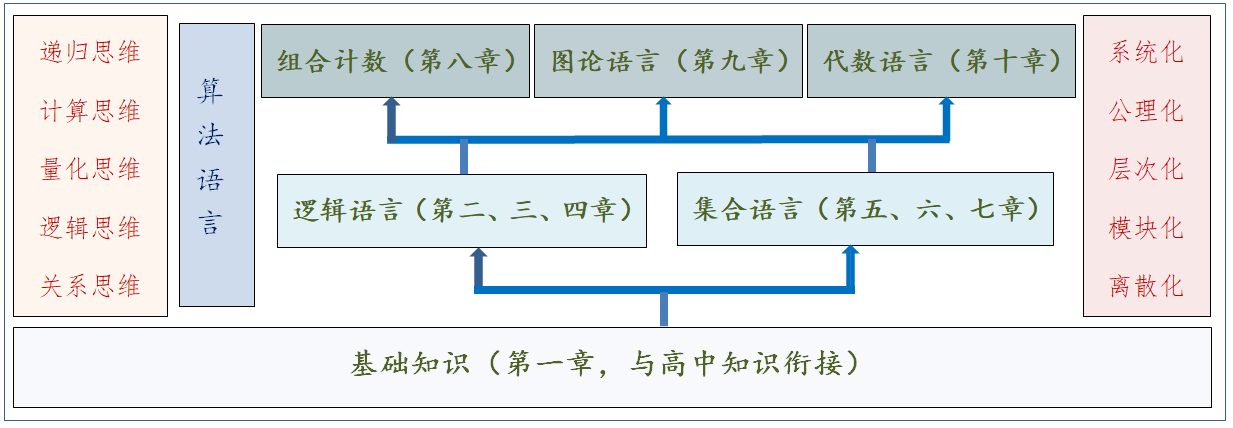
\includegraphics[width=0.72\textwidth]{\graphpath/bookframe.png} \else
\centering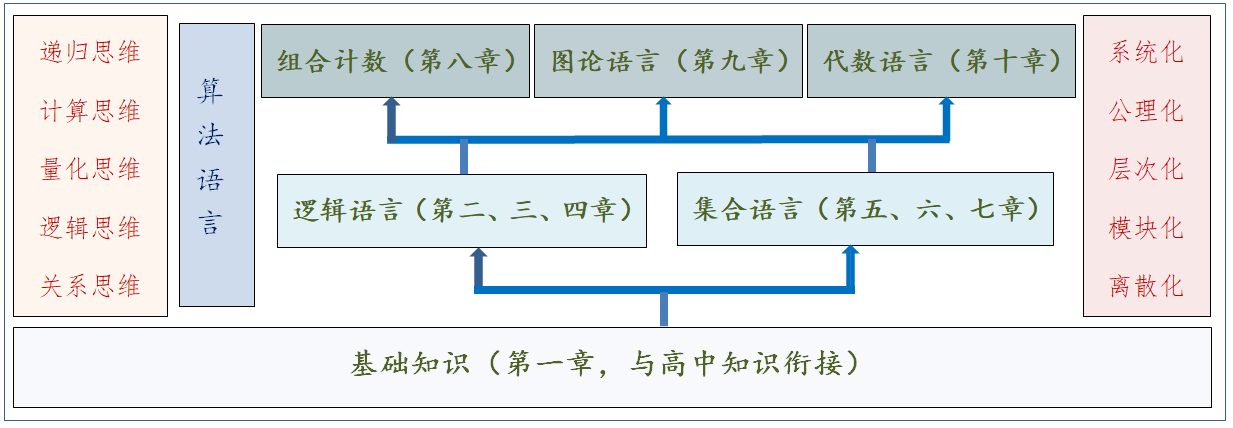
\includegraphics[width=0.72\textwidth,bb=0 0 1233 428]{\graphpath/bookframe.png} \fi
\caption{章节内容的整体框架结构}\label{figure:preface:book:frame}\vspace*{-0.8em}
\end{figure}

第一章“基础知识”给出有关逻辑语言、集合语言、图论语言、代数语言和算法语言的基础知识,这些基础知识大部分在中学学
习中已经接触,是对高中数学知识的衔接。这一章介绍这些离散数学语言的基本概念,并尽早地引入集合的归纳定义法、图的基
本概念、代数运算的基本概念以及算法的描述方法和算法的递归调用。这些内容在后面的章节中到处出现,是学习后面内容的准
备,后面要学习的内容则是这一章内容的拓展与深入。

第二章“命题逻辑”、第三章“一阶逻辑”和第四章“证明方法”属于逻辑语言的深入介绍。逻辑语言使用命题描述事物的性质
和事物之间的关系,核心的问题是确定命题的真值以及命题真值之间的关系,包括逻辑等值和逻辑推理关系。第二章学习命题逻
辑的基本概念、命题逻辑公式的语法和真值确定、命题逻辑公式的等值演算和基于命题逻辑公式的推理系统。第三章介绍有关一
阶逻辑的基本概念、一阶逻辑公式的语法和真值确定,一阶逻辑公式的等值演算和基于一阶逻辑公式的推理。第四章介绍基本的
证明方法,包括直接证明与间接证明、分情况证明、构造性与非构造性存在证明、数学归纳法、集合的归纳定义与结构归纳法。
通过第四章的学习,读者不仅可熟悉基本的数学证明方法和思路,提高自己的数学证明能力,而且可进一步体会逻辑语言的使用。

第五章“集合”、第六章“关系”和第七章“函数”属于集合语言的深入介绍。集合语言是现代数学的基本语言,使用集合、关
系、函数等描述所要研究的数学对象以及它们之间的联系。第五章介绍集合基本概念、集合运算、集合等式和子集关系证明。
第六章介绍关系的基本概念、关系运算、关系性质、关系的闭包,以及两种特殊的关系——等价关系和偏序关系。第七章介绍函
数的基本概念、函数性质和函数运算,并介绍集合等势、有穷集和无穷集、可数集和不可数集的基本知识,讨论函数的增长及
其在算法效率分析方面的应用和一些关于算法复杂度的基础知识。

逻辑语言和集合语言是学习组合计数、图论语言和代数语言的基础。第八章“计数与组合”介绍基本的组合计数原理、排列与组
合、二项式定理及二项式系数恒等式的证明、递推关系的构建与线性递推关系式的求解。第二、三、四章,特别是第四章的证明
体现逻辑思维的运用,而第五、六、七章,特别是第六章的关系和第七章的函数体现关系思维,第八章展示量化思维的运用,不
仅讨论集合元素的计数,而且进一步讨论算法效率的分析,特别是递归算法和分治算法的效率分析。

第九章“图与树”对图论语言做比较深入的介绍,在总结图和树基本概念的基础上,对图的连通性、图的遍历、树的遍历,以及
带权图的顶点间最短距离、最优二叉树、图的最小生成树等做更多的讨论,并对一些特殊的图,包括平面图、欧拉图、哈密顿
图做简单的介绍。

第十章“代数系统”对代数语言做比较深入的介绍,在定义运算及其性质的基础上,介绍代数系统的基本概念、代数的构造(子
代数、同余关系和商代数)、代数同态和同构,并介绍代数系统的例子,包括群、格与布尔代数的一些基础知识。

第十一章“结束语”,总结整个教材的内容,介绍可以进一步学习的离散数学相关知识,并给出一些推荐阅读的参考文献。

我们没有单列一章介绍算法的相关内容,但第一章的“基础知识”有一节专门介绍算法语言的基本知识,包括算法的基本概念和
基本特点,结合例子给出了如何使用结构化自然语言描述算法的顺序结构、选择结构和循环结构,以及算法调用的方法,并尽早
引入了递归调用和递归算法的概念。计算机专业的学生在学习离散数学时应注意思考如何利用计算机辅助求解离散数学的问题,
因此算法语言的使用和计算思维、递归思维的运用应该贯穿对逻辑、集合、图论和代数的学习,相关的章节也会给出许多算法的
例子。另外,第七章对函数的介绍会讨论函数的增长及其在算法效率分析中的应用,第八章的计数与组合会介绍递推关系式及其
在算法效率分析中的应用。

不少离散数学教材有关于数论的基础知识,我们没有单列一章介绍有关数论的基本知识,但不少内容,包括简单的算法例子、数
学问题的证明、计数与组合中都会有涉及整数性质的例子。这些例子会给出一些重要的数论基本知识,包括最大公因数及其
欧几里得算法、素数及素数的无穷性、两整数最大公因数的贝祖定理(B\'{e}zout's Theorem)等。

本书每一章的定义、定理和例子都分别按章跨节编号。我们只将能够严格使用数学语言定义,并且对于离散数学基础课程学习非
常重要的概念作为定义,定义的正文使用楷体以与其他正文区别,其中被定义的概念使用黑体。定理、引理和推论都沿用定理的
编号,给出每一章一些最重要的结论。我们精心挑选每一知识模块所需的定义和定理,使得它们能形成一个相对完整的整体,但
不至于有太多、太散的概念和结论需要读者记忆和学习。

我们将例子进一步分为例子和问题,例子主要用于进一步解释定义给出的概念或定理给出的结论,问题则偏向定义和定理的应
用,给出的问题在形式上与这一章的习题及运用离散数学要求解的实际问题相同,并且除给出参考的【解答】或【证明】外,通
常在解答前可能有【分析】部分介绍求解问题的思路和切入点,在解答后可能有【讨论】部分补充解答的一些注意事项以及
可能的启发。因此不少问题也适合用于翻转课堂教学模式中在学生自学章节主要内容之后进行的讨论式教学。

\begin{window}[0,r,{\mbox{%
\ifpdf 
\includegraphics[width=0.14\textwidth]{\graphpath/sample2Dcode.png} \else

\includegraphics[width=0.14\textwidth,bb=0 0 134 134]{\graphpath/sample2Dcode.png} \fi
}},{}]
本书每一章除给出大量例子和问题外,还给出了本章小结,总结这一章的主要概念和主要结论,以及学习这一章之后读者应该了解、
熟悉的概念以及应该能求解的问题。每一章的习题在这一章的最后一节给出,其中大部分习题用于巩固学习的内容,与这一章中
给出的问题十分类似,但也给出了一些扩展性的、有一定难度的习题,供基础好的读者练习,其中标记星号``*''的习题是推荐
的习题,可作为课后作业布置给学生完成。经过登记和验证的课程任课教师通过扫描这里旁边的二维码可获得习题的参考答案。
\end{window}

本书只假定学生有中学数学知识,如果已经接触过矩阵的基础知识,以及使用某门程序设计语言编写过计算机程序则更好。本书
可作为高等院校计算机相关专业本科一、二年级72学时至108学时的“离散数学基础”课程的教材,或者作为离散数学相关课程的
参考书,也可供从事计算机专业相关工作的科研人员、工程技术人员及其他有关人员参考。表\ref{table:prefrace:book:time}和
表\ref{table:prefrace:book:time2}给出了参考的课程学习计划和学时建议,其中列①针对周学时为4学时(总学时为72学
时)的课程,列②针对周学时为6学时(总学时为108学时)的课程(每学期上课周数设为18周),任课教师可根据情况选用。
本书对应表中列出的每个教学单元的起始点给出了二维码,扫描该二维码可获得该教学单元的课件和视频讲解等教学资源。

\begin{table}[!htb!p]
\caption{课程学习计划和学时建议}\label{table:prefrace:book:time}\zihao{-5}
\begin{tabular}{c|c|c|c|c|c}
\hline {\heiti 序}  & \centering{\heiti 教学单元} & \centering{\heiti 主要内容} & \centering{\heiti 选讲或略讲内容} & ① &  ② \\
\hline 1 & \tablecell{0.15\textwidth}{第一章} & \tablecell{0.3\textwidth}{基础知识:逻辑、集合、算法语言} & \tablecell{0.32\textwidth}{1.3 图论、1.4 代数语言} & 3 & 4 \\
\hline 2 & \tablecell{0.15\textwidth}{第二章2.1, 2.2, 2.3} & \tablecell{0.3\textwidth}{命题逻辑基本概念、命题逻辑公式的语法和语义} & \tablecell{0.32\textwidth}{2.2.2 命题逻辑公式的语法性质} & 2 & 3 \\
\hline 3 & \tablecell{0.15\textwidth}{第二章2.4} & \tablecell{0.3\textwidth}{命题逻辑等值演算} & \tablecell{0.32\textwidth}{2.4.3 命题逻辑公式的范式} & 2 & 3\\
\hline 4 & \tablecell{0.15\textwidth}{第二章2.5} & \tablecell{0.3\textwidth}{命题逻辑推理理论} & \tablecell{0.32\textwidth}{2.5.3 构造验证推理有效性的论证} & 2 & 3\\
\hline 5 & \tablecell{0.15\textwidth}{第二章2.6} & \tablecell{0.3\textwidth}{命题逻辑的应用} & \tablecell{0.32\textwidth}{2.6.3 算法性质的逻辑分析} & 2 & 3\\
\hline 6 & \tablecell{0.15\textwidth}{第三章3.1, 3.2, 3.3} & \tablecell{0.3\textwidth}{一阶逻辑基本概念、一阶逻辑公式的语法和语义} & \tablecell{0.32\textwidth}{3.3.1 一阶逻辑公式的解释} & 3 & 4\\
\hline 7 & \tablecell{0.15\textwidth}{第三章3.4} & \tablecell{0.3\textwidth}{一阶逻辑等值演算} & \tablecell{0.32\textwidth}{3.4.3 一阶逻辑的前束范式} & 2 & 3\\
\hline 8 & \tablecell{0.15\textwidth}{第三章3.5} & \tablecell{0.3\textwidth}{一阶逻辑的推理理论} & \tablecell{0.32\textwidth}{3.5.2 量词公式的推理规则} & 2 & 4\\
\hline 9 & \tablecell{0.15\textwidth}{第三章3.6} & \tablecell{0.3\textwidth}{一阶逻辑的应用} & \tablecell{0.32\textwidth}{3.6.3 算法性质的逻辑分析} & 2 & 3\\
\hline 10 & \tablecell{0.15\textwidth}{第四章4.1, 4.2} & \tablecell{0.3\textwidth}{直接证明、间接证明、分情况证明、存在性证明} & \tablecell{0.32\textwidth}{4.2.4 基本证明策略} & 3 & 4\\
\hline 11 & \tablecell{0.15\textwidth}{第四章4.3} & \tablecell{0.3\textwidth}{数学归纳法、良序原理、归纳定义、结构归纳法、递归算法} & \tablecell{0.32\textwidth}{4.3.1 数学归纳法与良序原理、4.3.3 递归算法与归纳证明} & 3 & 4\\
\hline 12 & \tablecell{0.15\textwidth}{第五章5.1, 5.2} & \tablecell{0.3\textwidth}{集合基本概念、集合运算} & \tablecell{0.32\textwidth}{5.1.3 文氏图与成员关系表、5.2.5 集合运算的算法} & 3 & 3\\
\hline 13 & \tablecell{0.15\textwidth}{第五章5.3} & \tablecell{0.3\textwidth}{集合等式} &    &    2 & 3\\
\hline 14 & \tablecell{0.15\textwidth}{第六章6.1} & \tablecell{0.3\textwidth}{关系定义、关系表示、关系运算} &   &     2 & 3\\
\hline 15 & \tablecell{0.15\textwidth}{第六章6.2} & \tablecell{0.3\textwidth}{关系性质} & \tablecell{0.32\textwidth}{6.2.4 关系性质与关系运算} & 2 & 3\\
\hline 16 & \tablecell{0.15\textwidth}{第六章6.3} & \tablecell{0.3\textwidth}{关系闭包} &      &  2 & 4\\
\hline 17 & \tablecell{0.15\textwidth}{第六章6.4} & \tablecell{0.3\textwidth}{特殊关系举例} &   &     2 & 3\\
\hline 18 & \tablecell{0.15\textwidth}{第七章7.1} & \tablecell{0.3\textwidth}{函数基本概念、性质和函数运算} & \tablecell{0.32\textwidth}{7.1.3 函数运算与函数性质} & 2 & 3\\
\hline 19 & \tablecell{0.15\textwidth}{第七章7.2} & \tablecell{0.3\textwidth}{集合等势、无穷集、可数集} & \tablecell{0.32\textwidth}{7.2.2 有穷集与无穷集} & 2 & 3\\
\hline 20 & \tablecell{0.15\textwidth}{第七章7.3} & \tablecell{0.3\textwidth}{函数的增长、算法效率分析} & \tablecell{0.32\textwidth}{7.3.3 算法复杂度基础知识} & 2 & 3\\
\hline 21 & \tablecell{0.15\textwidth}{第八章8.1} & \tablecell{0.3\textwidth}{加法原理、乘法原理、容斥原理、鸽笼原理} & \tablecell{0.32\textwidth}{8.1.3 鸽笼原理} & 3 & 4\\
\hline 22 & \tablecell{0.15\textwidth}{第八章8.2.1,\\8.2.2} & \tablecell{0.3\textwidth}{排列与组合、二项式定理、组合等式} &  &     2 & 4\\
\hline
\end{tabular}
\end{table}
\clearpage
\begin{table}[!htb!p]
\caption{课程学习计划和学时建议(续)}\label{table:prefrace:book:time2}\zihao{-5}
\begin{tabular}{c|c|c|c|c|c}
\hline {\heiti 序}  & \centering{\heiti 教学单元} & \centering{\heiti 主要内容} & \centering{\heiti 选讲或略讲内容} & ① &  ② \\
\hline 23 & \tablecell{0.15\textwidth}{第八章8.2.3,\\8.2.4, 8.2.5} & \tablecell{0.3\textwidth}{允许重复的排列与组合、容斥原理及其应用、排列组合的生成算法} & \tablecell{0.32\textwidth}{8.2.5 排列组合的生成算法} & 3 & 4\\
\hline 24 & \tablecell{0.15\textwidth}{第八章8.3} & \tablecell{0.3\textwidth}{递推关系式及其求解、分治算法与递推关系式} &   &     2 & 4\\
\hline 25 & \tablecell{0.15\textwidth}{第九章9.1} & \tablecell{0.3\textwidth}{图的基本概念、连通性、图的表示、无向图的遍历} & \tablecell{0.32\textwidth}{9.1.4 无向图的遍历} & 2 & 3\\
\hline 26 & \tablecell{0.15\textwidth}{第九章9.2} & \tablecell{0.3\textwidth}{树的基础知识} &    &    2 & 3\\
\hline 27 & \tablecell{0.15\textwidth}{第九章9.3} & \tablecell{0.3\textwidth}{带权图及其应用} &   &   2 & 4\\
\hline 28 & \tablecell{0.15\textwidth}{第九章9.4} & \tablecell{0.3\textwidth}{平面图、欧拉图、哈密尔顿图} &   &   2 & 3\\
\hline 29 & \tablecell{0.15\textwidth}{第十章10.1, 10.2} & \tablecell{0.3\textwidth}{运算及其性质、代数及同态} & \tablecell{0.32\textwidth}{10.2.2 同余关系与商代数} & 3 & 4\\
\hline 30 & \tablecell{0.15\textwidth}{第十章10.3} & \tablecell{0.3\textwidth}{群、子群、陪集、正规子群、商群} & \tablecell{0.32\textwidth}{10.3.2 群元素的阶、10.3.5 群同态} & 2 & 3\\
\hline 31 & \tablecell{0.15\textwidth}{第十章10.4} & \tablecell{0.3\textwidth}{格与布尔代数} & \tablecell{0.32\textwidth}{10.4.2 分配格与有界格} & 2 & 3\\
\hline  & & \tablecell{0.15\textwidth}{\heiti 总学时数} & &   70 & 105\\
\hline
\end{tabular}
\end{table}

本书编写过程中参考了许多国内外同类教材,得到了许多领导和老师的支持,在此对这些教材的编者以及支持我们的领导和老师
表示衷心的感谢。教材于2020年2月至7月在中山大学数据科学与计算机学院计算机大类四个教学班进行了试用,非常感谢参与的
老师和学生在试用的过程中提出了许多宝贵的意见和建议。这里还要特别感谢清华大学出版社的编辑,特别是白立军老师,没有
他们的耐心和支持,本书不可能得以出版。

在新工科建设背景下,基于培养计算机专业学生离散建模能力,编写一本与计算机专业其他课程,特别是与程序设计课程内容紧
密结合的离散数学教材是我们努力尝试的方向,但限于编者的水平,不一定达到了预期的目标。书中可能存在不少的疏漏和不妥
之处,恳请广大读者批评指正,并可随时与作者联系(isszxc@mail.sysu.edu.cn;~qiaohy@mail.sysu.edu.cn)。

~\\

\hfill 作~者~~\quad~\\

\hfill 2020~年~7~月~




%
